\documentclass[9pt,t,serif,professionalfont,xcolor={table,dvipsnames},noamsthm]{beamer}
\usepackage{xr-hyper}  % for cleveref; https://tex.stackexchange.com/a/244272/121234
\PassOptionsToPackage{pdfpagemode=FullScreen}{hyperref}
\setbeamersize{text margin left = 0.5cm,
               text margin right = 0.3cm}
\mode<presentation>
{
  \usetheme{boxes}
  \setbeamercovered{invisible}
  \setbeamertemplate{navigation symbols}{} 
}
\hypersetup{colorlinks=true,linkcolor=blue} 

\usepackage{../presentation,../presentationfonts}

% load the pdfanim style, should be done after hyperref
% \usepackage{pdfanim}

% load and initialise animation
% arguments:
%   \PDFAnimLoad[options]{name}{xxx}{number}
%   - options: in this example the animation is looped
%   - name: name of the animation
%     (with this name it can be reused several times in the document)
%   - number: number of animation frames / files (n)
% the animation will be composed of files
% xxx0.pdf, xxx1.pdf ... xxx(n-1).pdf


\title{Cardinality}

\author{Jim Hef{}feron}
\institute{
  Mathematics and Statistics\\
  Saint Michael's College\\
  Colchester, VT\\[1ex]
  \texttt{jhefferon@smcvt.edu}
}
\date{}

% This is only inserted into the PDF information catalog.
\subject{Cardinality}

\usepackage{catchfilebetweentags} % read text from background.tex
\newcommand{\catchfilefn}{../../background/background.tex}
% Keep from swallowing end-of-lines
%   https://tex.stackexchange.com/a/40704/121234
\usepackage{etoolbox}
\makeatletter
\patchcmd{\CatchFBT@Fin@l}{\endlinechar\m@ne}{}
  {}{\typeout{Unsuccessful patch!}}
\makeatother

\usepackage{xr}
  \externaldocument{../../book.aux}
\usepackage{cleveref}

\usepackage{multirow,bigstrut}
\begin{document}
\begin{frame}
  \titlepage
\end{frame}




\section{Cardinality}
% ------------------------------------------------------
\begin{frame}
  \frametitle{Finite sets have the same size iff there is a correspondence}
\begin{center}\small\setlength{\bigstrutjot}{30pt}
  \hspace*{-4em}% table looks funny else
  \begin{tabular}{rr|c@{\hspace*{3em}}c}
    \multicolumn{2}{c}{} &\multicolumn{2}{c}{\textit{One-to-one?}}  \\
    \multicolumn{2}{c}{} &\textit{No}  &\textit{Yes}   \\ \cline{3-4}
   \multirow{2}[2]{*}{\it Onto?}
   &\textit{No}
    &\bigstrut\vcenteredhbox{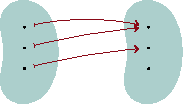
\includegraphics{asy/background02.pdf}} 
    &\vcenteredhbox{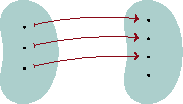
\includegraphics{asy/background01.pdf}}     \\
   &\textit{Yes}
    &\bigstrut\vcenteredhbox{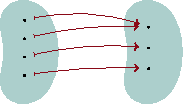
\includegraphics{asy/background00.pdf}} 
    &\vcenteredhbox{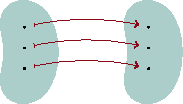
\includegraphics{asy/background03.pdf}}  \\
  \end{tabular}
\end{center}

\ExecuteMetaData[\catchfilefn]{lem:OneToOneOntoFiniteSets}
\end{frame}


\begin{frame}
  \frametitle{Cardinality definition}
\ExecuteMetaData[\catchfilefn]{lem:EquinumerosityIsEquivalence}

\pause
\ExecuteMetaData[\catchfilefn]{def:Cardinality}
\begin{center}
  \vcenteredhbox{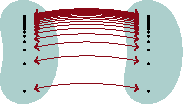
\includegraphics{asy/background04.pdf}} 
\end{center}

\pause
\begin{example}
These have the same cardinality:
(a)~$|A|=|B|$ where 
$A=\set{x\in\R\suchthat 0\leq x<1}$
and $B=\set{x\in\R\suchthat 1\leq x<5}$
(b)~$|C|=|D|$ where 
$C=\set{x\in\N\suchthat 0\leq x<10}$
and $D=\set{x\in\N\suchthat 1\leq x<11}$.
If $I=\set{x\in\R\suchthat 0<x<1}$ then $|I|=|\R|$
and if $S=\set{x\in\N\suchthat \text{$x$ is a square}}$ then $|S|=|\N|$.
\end{example}

\pause
\ExecuteMetaData[\catchfilefn]{def:FiniteInfinite}
\ExecuteMetaData[\catchfilefn]{def:Countable}
\ExecuteMetaData[\catchfilefn]{Enumeration}
\end{frame}


\begin{frame}
\begin{example}
The set $\set{n^2\suchthat n\in\N}$ is countably infinite.
It is enumerated by the function $\map{f}{\N}{\N}$ given by $f(x)=x^2$.
\end{example}

\begin{example}
The set $\N-\set{0,1,2}=\set{3,4,5,6,7,\ldots}$ is countably infinite.
The function $f(x)=x+3$ closes the gap.
\begin{equation*}
  \begin{array}{r|ccccccc@{\hspace{6pt}}c}
    n
      &0 &1 &2 &3 &4 &5 &6 &\ldots \\ \cline{2-9}
    f(n)
      &3
      &4
      &5
      &6
      &7
      &8
      &9
      &\ldots
  \end{array}
  \qquad    
\end{equation*}
This function is clearly one-to-one and onto.
\end{example}

\ExecuteMetaData[\catchfilefn]{ex:SetOfPrimesCountable}
\ExecuteMetaData[\catchfilefn]{ex:SetOfIntegersCountable}
\end{frame}

\begin{frame}
  \frametitle{Cross product}
\begin{example}
If $N_2=\set{0,1}\times\N$ then $|N_2|=|\N|$.
\begin{center}
  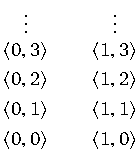
\includegraphics{../../background/asy/correspondences/correspondences1000.pdf}
\end{center}
\ExecuteMetaData[\catchfilefn]{table:CantorsCorrespondence}
\ExecuteMetaData[\catchfilefn]{def:PairingFcn}
\end{example}

\begin{example}
If $N_3=\set{0,1,2}\times\N$ then $|N_3|=|\N|$.
For any finite~$k$, 
if $N_k=\set{0,1,\ldots k-1}\times\N$ then $|N_k|=|\N|$.
\end{example}
\ExecuteMetaData[\catchfilefn]{lem:CrossProdFiniteCountableIsCountable}
\end{frame}


\begin{frame}
  \frametitle{Cantor's correspondence}
We next want to enumerate this array that is unbounded in two dimensions.
\ExecuteMetaData[\catchfilefn]{eqn:TwoByTwoArray}
\pause
\ExecuteMetaData[\catchfilefn]{table:CantorsCorrespondence}
\ExecuteMetaData[\catchfilefn]{def:CantorsCorrespondence}
\pause
\ExecuteMetaData[\catchfilefn]{lem:CantorsCorrespondenceIsCorrespondence}
\ExecuteMetaData[\catchfilefn]{cor:CroosProdFinitelyManyCountablyManyIsCountable}
\end{frame}





%========================================
\section{Enumerating Turing machines}

\begin{frame}
  \frametitle{Counting Turing machines}
\ExecuteMetaData[\catchfilefn]{def:NumberingTMs}
Fix some acceptable numbering that we will use for the rest of the course.
\pause
\ExecuteMetaData[\catchfilefn]{lem:EachTMHasInfManyIndices}
\end{frame}



\begin{frame}
  \frametitle{A way to informally think about numbering}
Turing machines are like programs.
Imagine that you have a program $\TM$ in your editor, and save it to disc.
It gets put on the hard drive as a bit string, 
which you can think of as a number~$e$ written in binary.
The operating system associates  
from program to number and from number to program.
Both associations are effective, since the operating system is a program.
\begin{center}
  \includegraphics{asy/background05.pdf}
\end{center}
\pause
This is only an analogy\Dash for instance leading \str{0}'s
in the bit string cause ambiguity\dash but like any analogy its
point is to help us get a better sense of what is happening.
A Turing machine's index number is a name, a way to refer to that machine.
We can go from machine source to index, or from index to machine source,
effectively.
\end{frame}





\section{Diagonalization}

\begin{frame}
  \frametitle{There are sets that are uncountable}
\ExecuteMetaData[\catchfilefn]{th:NoOntoMapNToR}
\ExecuteMetaData[\catchfilefn]{table:EnumerateR}
\pause
\ExecuteMetaData[\catchfilefn]{pf:NoOntoMapNToR}
\end{frame}


\begin{frame}
  \frametitle{Uncountable sets}

\ExecuteMetaData[\catchfilefn]{def:Uncountable}
\begin{example}
We can adjust the argument to show that there is no onto function 
from $\N$ to $S$ where:
(a)~$S=\R^+=\set{x\in\R\suchthat x>0}$
(b)~$S=\leftclosed{0}{1}$,
\end{example}

\ExecuteMetaData[\catchfilefn]{def:CardLessThanOrEqual}
\begin{example}
We have $|\N|\leq |\R|$, and in fact 
by the result above it is strictly less than.
\end{example}
\end{frame}



\begin{frame}
  \frametitle{Cantor's Theorem}
\ExecuteMetaData[\catchfilefn]{recall:CharFcn}

\ExecuteMetaData[\catchfilefn]{th:CantorsThm}
\ExecuteMetaData[\catchfilefn]{ex:CantorsThm}
\end{frame}


\begin{frame}
\ExecuteMetaData[\catchfilefn]{th:CantorsThm}
\ExecuteMetaData[\catchfilefn]{pf:CantorsThm}
\end{frame}



\begin{frame}
  \frametitle{There are uncomputable sets}

\ExecuteMetaData[\catchfilefn]{cor:FcnsNToNNotCountable}
\ExecuteMetaData[\catchfilefn]{pf:FcnsNToNNotCountable}

\pause
Turing machines compute functions from $\N$ to $\N$.
There are uncountably many such functions, but only countably many 
Turing machines.
Thus there are function that are not computed by any Turing machine.

This is like Musical Chairs.
There are a smaller number of chairs (Turing machines) than children
(functions from $\N$ to~$\N$).
When the music stops some children are left without a chair, and similarly
some functions have no associated Turing machine.

\pause
\vspace*{2ex}
\fbox{\parbox{\dimexpr\textwidth-2\fboxsep-2\fboxrule\relax}{%
  \color{red}
  In the light of Church's Thesis we interpret this as:~there are jobs 
  that no computer can do.}}
\end{frame}



\section{Universality}

\begin{frame}
  \frametitle{Universal Turing machine}
\ExecuteMetaData[\catchfilefn]{th:UniversalTM}
\ExecuteMetaData[\catchfilefn]{discussion:UniversalTM}

\begin{itemize}
\item A $\UTM$ is like an interpreter, or like an operating system. 
\item This converts doing jobs in hardware job to doing them in software.
\item The universal machine does not get as input a Turing machine, it gets
  the index of a Turing machine, which is equivalent to the
  a representation of that machine.
\item Yes, we could feed the $\UTM$ a representation of itself.
\end{itemize}
\end{frame}





% ====================================================
\section{The \protect\smn~Theorem}


\begin{frame}[fragile]
  \frametitle{Partial evaluation}

Start with a two-input function.

\begin{lstlisting}
def power(base, exponent):
    return base ** exponent  
\end{lstlisting}

By freezing, or parametrizing, 
one if its arguments we get a family of functions.

\begin{lstlisting}
def power_1(base):    # identity function
    return power(base, 1)
def power_2(base):    # squaring function
    return power(base, 2)
def power_3(base):    # cubing function
    return power(base, 3)
\end{lstlisting}

\pause
Python has a more systemmatic way to accomplishes the same thing.

\begin{lstlisting}
from functools import partial
power_1 = partial(power, exponent=1)
power_2 = partial(power, exponent=2)
power_3 = partial(power, exponent=3)
\end{lstlisting}
\end{frame}



\begin{frame}[fragile]
  \frametitle{Freezing variables}

On the left is a three input routine.
By Church's Thesis there is a Turing machine to do the same behavior;
let its index be~$e$.
\begin{center}
  \vcenteredhbox{\includegraphics{asy/background06.pdf}}
  \hspace{3em}
  \vcenteredhbox{\includegraphics{asy/background07.pdf}}
\end{center}
On the right we have frozen the first two inputs.
The \smn~Theorem, which we are about to see,
says that we can do this uniformily:~there is a program that takes in
$e$, $5$, and~$7$ and outputs the index of the Turing machine 
on the right. 

Further, it says that a single program works in all
leave $1$-input, freeze the other~$2$ situations.
We write $s_2^{1}$ for the function that is the behavior of that program.
In this class we will usually
just call that function~$s$:
\begin{center}
  \parbox{0.7\textwidth}{Where $e$ is the index of the Turing machine on the left,
$s(e,5,7)$ is the index of the machine on the right.}
\end{center}
\end{frame}




\begin{frame}
    \frametitle{Parametrization}

Universality says that there is a computable
function $\map{F}{\N^2}{\N}$ such that
$F(e,x)=\phi_e(x)$.
There, the letter~$e$ travels from the function's argument to an index.

\ExecuteMetaData[\catchfilefn]{th:smn}

This is the \alert{\smn~Theorem} or 
\alert{Parametrization Theorem}.

\pause
\textsc{Pf.}
\ExecuteMetaData[\catchfilefn]{pf:smni}
\end{frame}


\begin{frame}
\begin{center}
  \vcenteredhbox{\includegraphics{../../background/asy/flowcharts/flowcharts00.pdf}}
  \hspace{3em}
  \vcenteredhbox{\includegraphics{../../background/asy/flowcharts/flowcharts01.pdf}}
\end{center}
\ExecuteMetaData[\catchfilefn]{pf:smnii}\qedsymbol
\end{frame}



\begin{frame}{A family of functions}
Recall again the \lstinline{power} routine.

% \begin{lstlisting}
% def power(base, exponent):
%     return base ** exponent  
% \end{lstlisting}

\begin{center}
  \vcenteredhbox{\includegraphics{asy/background08.pdf}}
\end{center}

Suppose that is the machine with index~$e$.
Looking at the different machines indexed by $s(e,x)$ 
gives a family of routines.

% \begin{lstlisting}
% def identity(base):
%     return power(base, 1)
% def square(base):
%     return power(base, 2)
% def cube(base):
%     return power(base, 3)
% \end{lstlisting}

\begin{center}
  \vcenteredhbox{\includegraphics{asy/background09.pdf}}
  \hspace{1em}
  \vcenteredhbox{\includegraphics{asy/background10.pdf}}
  \hspace{1em}
  \vcenteredhbox{\includegraphics{asy/background11.pdf}}
  \hspace{1em}
  \ldots
  \hspace{1em}
  \vcenteredhbox{\includegraphics{asy/background12.pdf}}
  \hspace{1em}
  $\ldots$
\end{center}
\end{frame}




% ====================================================
\section{The \HP}


\begin{frame}
  \frametitle{\HP}
We are interested in finding which things are mechanically computable.
We effectivize Cantor's Theorem.
This is the table from the discussion leading to that result.
\begin{center}
  \ExecuteMetaData[\catchfilefn]{table:CantorThmEffectivization}
  \hspace*{2em plus 0.75fil}
  \vcenteredhbox{\includegraphics{../../background/asy/hp/hp02.pdf}}
\end{center}
Consider the flowchart on the right.
All the boxes except the middle one are trivial.
For the middle, use universality to simulate Turing machine~$e$ 
running input~$e$.

\pause
But wait, that looks like a program giving output that isn't on the list
of all program outputs.
Where is the flaw in the reasoning?

\pause
Inherent in the nature of mechanical computation, necessary to avoid
contradiction, is that some computations fail to halt.
\end{frame}


\begin{frame}
\ExecuteMetaData[\catchfilefn]{def:K}

In the notation of effective functions it is 
$K=\set{e\suchthat \TMfcn_e(e)\converges}$.

\ExecuteMetaData[\catchfilefn]{prob:HP}

This is the \alert{\HP}.
\pause
\ExecuteMetaData[\catchfilefn]{th:HPIsUnsolvable}

\textsc{Pf.} \ExecuteMetaData[\catchfilefn]{pf:HPIsUnsolvablei}
\begin{center}
\begin{minipage}{0.3\textwidth}
  \begin{equation*}
  f(e)=
    \begin{cases}
    0    &\case{if $\TMfcn_e(e)\diverges$}  \\
    \uparrow  &\case{if $\TMfcn_e(e)\converges$}
    \end{cases}
  \end{equation*}
\end{minipage}
\hspace{2.5em}
\vcenteredhbox{\includegraphics{../../background/asy/flowcharts/flowcharts02.pdf}}
\end{center}
\end{frame}



\begin{frame}
\ExecuteMetaData[\catchfilefn]{pf:HPIsUnsolvableii}\qedsymbol
\end{frame}



\begin{frame}[fragile]
  \frametitle{Discussion: the \HP{} is unsolvable}

\begin{itemize}
\item ``Unsolvable'' means unsolvable by a Turing machine.
  This is a perfectly good function that solves the \HP.
  \begin{equation*}
    \computablefunction{halt\_checker}(e)=
    \begin{cases}
      1  &\case{if $\TMfcn_e(e)\converges$}  \\
      0  &\case{if $\TMfcn_e(e)\diverges$}  \\
    \end{cases}
  \end{equation*}
  However no Turing machine has this behavior.

\item
Unsolvability of \HP{} 
does not mean that for no program can we tell if that program halts, 
nor does it mean that for no program can we tell that the program does not halt.
The program on the left halts, no matter what is the input.
The program on the right does not halt, no matter what the input.
\begin{center}
% \vspace*{-4ex}
\vspace*{-\ht\strutbox}
\begin{minipage}[t]{0.4\linewidth}%
\begin{lstlisting}
read x
print x
\end{lstlisting}%
\end{minipage}%
\hspace*{2em plus 0.5fil}
\begin{minipage}[t]{0.4\linewidth}%
\begin{lstlisting}
read x
while True:
    x = x+1
print x
\end{lstlisting}%
\end{minipage}%
\end{center}

\item
Instead, the unsolvability of the Halting Problem 
says that there is no single program that, for all input~$e$, 
correctly computes in a finite time whether $\TM_e$ halts on~$e$.
\end{itemize}
\end{frame}

\begin{frame}[fragile]{Discussion continued}
\begin{itemize}
\item \textit{The unsolvability of the Halting Problem 
  says that there is no single program that, for all~$e$, correctly computes 
  in a finite time whether $\TM_e$ halts on input~$e$.}
  The ``finite time'' qualifier is there because we could just use a universal
  Turing machine to simulate $\TM_e$ on~$e$, but if that machine failed to halt
  then we would not find out in a finite time. 
  The ``single program'' qualifier is there because for any index~$e$,
  either $\TM_e$ halts on~$e$ or it does not.
  That is, for any~$e$ one of these two programs
  gives the right answer.
\begin{center}
% \vspace*{-4ex}
\vspace*{-\ht\strutbox}
\begin{minipage}[t]{0.4\linewidth}%
\begin{lstlisting}
read e
print 0
\end{lstlisting}%
\end{minipage}%
\hspace*{2em plus 0.5fil}
\begin{minipage}[t]{0.4\linewidth}%
\begin{lstlisting}
read e
print 1
\end{lstlisting}%
\end{minipage}%
\end{center}

\item
Thus, the unsolvability of the Halting Problem is about 
the non-existence of a single program that works across all
indices.
It speaks to uniformity,
or rather, the impossibility of uniformity.
\end{itemize}
\end{frame}



\begin{frame}
  \frametitle{Unsolvability via reduction to \HP}

Each of these problems is unsolvable.  
For each, we show that by using \HP.

\begin{enumerate}
\item The problem of determining whether a given Turing machine
  halts on input~$1$.
  \begin{equation*}
    \computablefunction{halts\_on\_one\_checker}(e)=
    \begin{cases}
      1  &\case{if $\TMfcn_e(1)\converges$}  \\
      0  &\case{otherwise}
    \end{cases}
  \end{equation*}
\item The problem of determining whether a given Turing machine ever
  outputs a 19.
  \begin{equation*}
    \computablefunction{outputs\_nineteen\_checker}(e)=
    \begin{cases}
      1  &\case{if there is $x$ such that $\TMfcn_e(x)=19$}  \\
      0  &\case{otherwise}
    \end{cases}
  \end{equation*}
\item The problem of determining whether a given Turing machine 
  gives as output the square of its input.
  \begin{equation*}
    \computablefunction{ever\_squares\_checker}(e)=
    \begin{cases}
      1  &\case{if there is $x$ such that $\TMfcn_e(x)=x^2$}  \\
      0  &\case{otherwise}
    \end{cases}
  \end{equation*}
\end{enumerate}
\end{frame}


\begin{frame}
  \frametitle{Rice's Theorem}
\ExecuteMetaData[\catchfilefn]{def:SameBehavior}
\ExecuteMetaData[\catchfilefn]{def:IndexSet}

\begin{example}
These are index sets:
(1)~$\set{e\in\N\suchthat
      \text{$\phi_e(x)=9$}}$
(2)~$\set{e\in\N\suchthat
      \text{$\phi_e(x)=2x$ or $\phi_e(x)=x+6$}}$
and (3)~$\set{e\in\N\suchthat
      \text{$\phi_e(1)\converges$}}$
\end{example}

\pause
\ExecuteMetaData[\catchfilefn]{th:RicesTheorem}

\textsc{Pf.}
\ExecuteMetaData[\catchfilefn]{pf:RicesTheoremi}
\end{frame}


\begin{frame}
\begin{center}
  \vcenteredhbox{\includegraphics{../../background/asy/hp/hp12.pdf}}
  \hspace{2em plus 0.5fil}
  \vcenteredhbox{\includegraphics{../../background/asy/hp/hp13.pdf}}
\end{center}
\ExecuteMetaData[\catchfilefn]{pf:RicesTheoremii}\qedsymbol

\pause
Show each of these is unsolvable using Rice's Theorem.

\begin{enumerate}
\item The problem of determining whether a given Turing machine
  halts on input~$1$.
\item The problem of determining whether a given Turing machine ever
  outputs a 19.
\item The problem of determining whether a given Turing machine 
  gives as output the square of its input.
\end{enumerate}
\end{frame}








% ====================================================
\section{Computably enumerable sets}

\begin{frame}[fragile]
\ExecuteMetaData[\catchfilefn]{def:ComputableSet}
\ExecuteMetaData[\catchfilefn]{def:ComputablyEnumerable}

Picture a stream of numbers generated by a computable function
$\TMfcn_e(0)$, $\TMfcn_e(1)$, $\TMfcn_e(2)$,~\ldots{}\@
Note that a computably enumerable set can be empty, if
$\TMfcn_e$ never converges.

\begin{example}
These are computably enumerable:
(i)~$\set{1,3,5}$,
(ii)~$\set{2n\suchthat n\in\N}$,
(iii)~$\set{y\suchthat\text{there is an $x$ so that $y=\TMfcn_{19}(x)$}}$,
(iv)~$\set{x\suchthat\TMfcn_{19}(x)\converges}$.
\end{example}
\end{frame}

\begin{frame}[fragile]
\ExecuteMetaData[\catchfilefn]{description:DecidableAndSemidecidable}

\pause
\begin{lemma}
\ExecuteMetaData[\catchfilefn]{lem:ComputableAndCEi}
\ExecuteMetaData[\catchfilefn]{lem:ComputableAndCEii}
\end{lemma}

\ExecuteMetaData[\catchfilefn]{lem:HPIsCE}

% \ExecuteMetaData[\catchfilefn]{lem:CEIffDomainOfComputableFcn}
\end{frame}






% =====================================================
\section{Fixed point theorem}

\begin{frame}
  \frametitle{When diagonalization fails}

\ExecuteMetaData[\catchfilefn]{discussion:RecallCantorThm}

\pause
\ExecuteMetaData[\catchfilefn]{discussion:WhenDiagonalizationFails}
\end{frame}


\begin{frame}
\ExecuteMetaData[\catchfilefn]{discussion:WhenDiagonalizationFailsii}
\end{frame}


\begin{frame}
\begin{theorem}
\ExecuteMetaData[\catchfilefn]{th:FixedPointThm}
\end{theorem}

\pause
\textsc{Pf.}
\ExecuteMetaData[\catchfilefn]{pf:FixedPointThmi}
\begin{equation*}
  \vcenteredhbox{\includegraphics{../../background/asy/flowcharts/flowcharts06.pdf}}
  \hspace{1em}
  \vcenteredhbox{\includegraphics{../../background/asy/flowcharts/flowcharts07.pdf}}
  \hspace{2em}
  d_n(x)=
  \begin{cases}
    \TMfcn_{\TMfcn_n(n)}(x)  &\case{if $\TMfcn_n(n)\converges$} \\
    \uparrow                &\case{otherwise}
  \end{cases}
\end{equation*}
\end{frame}



\begin{frame}
\ExecuteMetaData[\catchfilefn]{pf:FixedPointThmii}
\begin{equation*}
  t_f(d_n)\;(x)=
  \begin{cases}
    \TMfcn_{f\TMfcn_n(n)}(x)   &\case{if $\TMfcn_n(n)\converges$}     \\
    \uparrow                 &\case{otherwise}
  \end{cases}
  \hspace{2em}
  \vcenteredhbox{\includegraphics{../../background/asy/flowcharts/flowcharts08.pdf}}
\end{equation*}
\ExecuteMetaData[\catchfilefn]{pf:FixedPointThmiii}\qedsymbol
\end{frame}



\begin{frame}
\ExecuteMetaData[\catchfilefn]{cor:WeEqualsSete}

\textsc{Pf.}
\ExecuteMetaData[\catchfilefn]{pf:WeEqualsSetei}
\begin{equation*}
  \vcenteredhbox{\includegraphics{../../background/asy/flowcharts/flowcharts09.pdf}}
  \hspace{1em}
  \vcenteredhbox{\includegraphics{../../background/asy/flowcharts/flowcharts10.pdf}}
  \hspace{1em}
  \TMfcn_{s(e_o,m)}(x)=
  \begin{cases}
  0         &\case{if $x=m$}  \\
  \uparrow  &\case{otherwise}
  \end{cases}
\end{equation*}
\ExecuteMetaData[\catchfilefn]{pf:WeEqualsSeteii}\qedsymbol
\end{frame}

\end{document}




